\documentclass[tikz,border=6pt]{standalone}
\usepackage{amsmath}
\usetikzlibrary{arrows.meta,positioning}

\definecolor{condfill}{RGB}{230,240,255}
\definecolor{condstroke}{RGB}{74,111,165}
\definecolor{margfill}{RGB}{246,238,220}
\definecolor{margstroke}{RGB}{156,119,65}
\definecolor{arrowgray}{RGB}{90,98,110}

\begin{document}
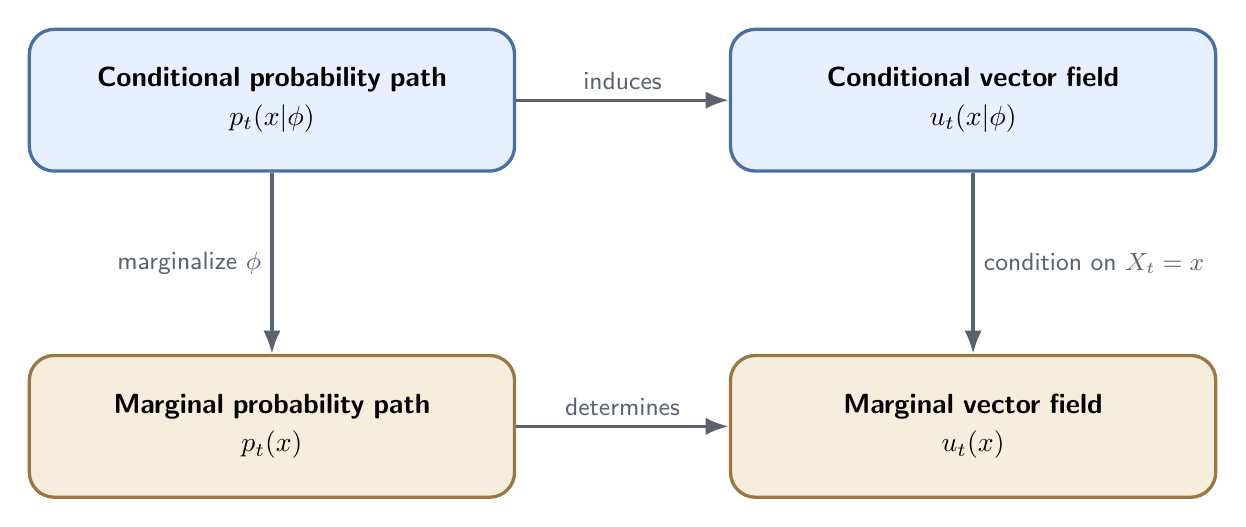
\begin{tikzpicture}[
  font=\sffamily,
  >=Latex,
  node distance=2.3cm and 2.7cm,
  theorybox/.style={
    rounded corners=9pt,
    draw,
    very thick,
    text width=5.6cm,
    minimum height=1.8cm,
    align=center,
    inner sep=8pt
  },
  cond/.style={theorybox, draw=condstroke, fill=condfill},
  marg/.style={theorybox, draw=margstroke, fill=margfill},
  flowarrow/.style={->, very thick, draw=arrowgray},
  maplabel/.style={font=\small\sffamily, text=arrowgray}
]

\node[cond] (cp) {\textbf{Conditional probability path}\\[2pt]$p_t(x|\phi)$};
\node[cond, right=of cp] (cv) {\textbf{Conditional vector field}\\[2pt]$u_t(x|\phi)$};
\node[marg, below=of cp] (mp) {\textbf{Marginal probability path}\\[2pt]$p_t(x)$};
\node[marg, below=of cv] (mv) {\textbf{Marginal vector field}\\[2pt]$u_t(x)$};

\draw[flowarrow] (cp) -- node[maplabel, above] {induces} (cv);
\draw[flowarrow] (mp) -- node[maplabel, above] {determines} (mv);
\draw[flowarrow] (cp) -- node[maplabel, left] {marginalize $\phi$} (mp);
\draw[flowarrow] (cv) -- node[maplabel, right] {condition on $X_t=x$} (mv);

\end{tikzpicture}
\end{document}
